\graphicspath{{lectures/1axioms/asy/}}

\pagestyle{empty}

\subsection*{Worksheet: Squares, Parallelograms and Area}

To prove Pythagoras' Theorem, Euclid needs to compare areas of triangles and parallelograms, and to construct squares. Prove the following as best as you can: the pictures will help!
\begin{enumerate}
\begin{minipage}[t]{0.6\linewidth}\vspace{0pt}
	\item (Thm I.\,11) At a given point $A$ on a line $\cl{AB}$, to construct a perpendicular.
\end{minipage}\begin{minipage}[t]{0.4\linewidth}\vspace{0pt}
	\flushright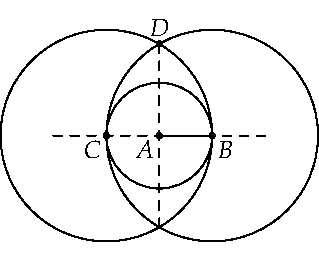
\includegraphics{euclid-I11}
\end{minipage}
	
	\vfill
	
	\begin{minipage}[t]{0.6\linewidth}\vspace{0pt}
	\item (Thm I.\,46) To construct a square on a given segment.
\end{minipage}\begin{minipage}[t]{0.4\linewidth}\vspace{0pt}
	\flushright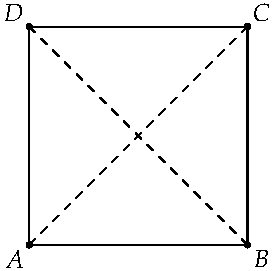
\includegraphics{euclid-I46}
\end{minipage}

\vfill\newpage

	\item (Thm I.\,35) Parallelograms $\square ABCD$ and $\square ABEF$ on the same base and with the same height have equal area.
	\begin{center}
	\begin{tabular}{ccc}
	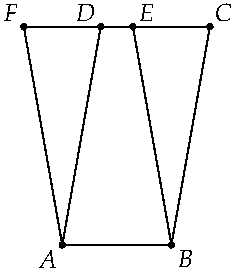
\includegraphics{euclid-I35a}&\qquad\qquad\qquad&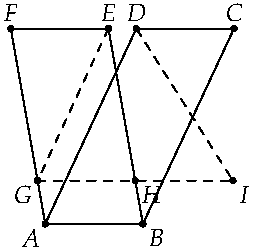
\includegraphics{euclid-I35}\\
	Case 1&&Case 2
	\end{tabular}
	\end{center}
	
	\vfill\vfill
	
	\item (Thm I.\,41) A parallelogram has twice the area of a triangle on the same base and with the same height.
\end{enumerate}

\vfill
	
